% Figi H : kalandriye previzyonèl egzekisyon pwojè a, 16 novanm 2026 -> 15 janvye 2027.
% Jou 0 = lendi 16 novanm 2026 ; yon jou = 0,2213 cm. De check-in pa semèn (madi ak jedi).
\documentclass[tikz,border=4pt]{standalone}
% Stil komen pou tout figi yo (xelatex). Figi yo trase a gwosè reyèl (17 cm lajè),
% konsa tèks yo rete lizib lè yo antre nan pwopozisyon an san rediksyon.
\usepackage{fontspec}
\setmainfont{FiraSans}[Extension=.otf, UprightFont=*-Regular, BoldFont=*-SemiBold,
  ItalicFont=*-Italic, BoldItalicFont=*-BoldItalic]
\newfontfamily\headfont{Montserrat}[Extension=.otf, UprightFont=*-Bold, BoldFont=*-ExtraBold]
\usepackage{fontawesome5}
\usetikzlibrary{arrows.meta, calc, shadows.blur, shapes.symbols, decorations.pathreplacing}
\graphicspath{{../../assets/logos/}{../../assets/}}

% Palèt logo APA a
\definecolor{apablue}{HTML}{3D61E9}
\definecolor{apacoral}{HTML}{FF485E}
\definecolor{apayellow}{HTML}{FEDE44}
\definecolor{apaink}{HTML}{1F2937}
\definecolor{apagray}{HTML}{6B7280}
\definecolor{apaline}{HTML}{D6DAE1}

\newif\ifapahl % true = mete aksan sou etap 1 an (vèsyon Faz pa faz)

\newcommand{\lbl}[1]{{\fontsize{7.8pt}{9pt}\selectfont\bfseries\color{apaink}#1}}
\newcommand{\sub}[1]{{\fontsize{6.6pt}{7.8pt}\selectfont\color{apagray}#1}}
\newcommand{\body}[1]{{\fontsize{7.6pt}{9.4pt}\selectfont\color{apaink}#1}}
\newcommand{\lgo}[2][0.58cm]{\includegraphics[height=#1,width=0.75cm,keepaspectratio]{#2}}
% httpx2 pa gen logo : yon badj tèks, jamè papiyon ansyen httpx la
\newcommand{\httpxbadge}[1][7.4pt]{{\setlength{\fboxsep}{2.4pt}%
  \colorbox{apaink}{\headfont\fontsize{#1}{#1}\selectfont\color{white}HTTPX2}}}

\tikzset{
  card/.style={draw=apaline, line width=0.5pt, fill=white, rounded corners=5pt,
    blur shadow={shadow blur steps=6, shadow xshift=0.5pt, shadow yshift=-0.7pt,
      shadow opacity=22}, align=center, inner sep=3pt},
  flow/.style={-{Stealth[length=5.5pt, width=4.5pt]}, line width=0.95pt, color=apaink!75},
  dflow/.style={flow, dashed, color=apagray},
  key/.style={densely dotted, line width=0.8pt, color=apagray},
  pill/.style={rounded corners=4pt, inner xsep=4pt, inner ysep=2pt,
    font=\fontsize{7.2pt}{8pt}\selectfont\bfseries},
  badge/.style={circle, inner sep=1.3pt, fill=apacoral, text=white,
    font=\fontsize{6.2pt}{6.2pt}\selectfont},
  num/.style={circle, inner sep=0pt, minimum size=0.42cm,
    font=\headfont\fontsize{8pt}{8pt}\selectfont},
}

% Kat orizontal : logo a goch, tèks a dwat.
% \hcard[opsyon]{non}{pozisyon}{lajè}{logo}{etikèt}{sou-etikèt}
\newcommand{\hcard}[7][]{%
  \node[card, minimum width=#4, minimum height=1.0cm, #1] (#2) at (#3) {};
  \node at ($(#2.west)+(0.47,0)$) {#5};
  \node[anchor=west, align=left, inner sep=0pt] at ($(#2.west)+(0.88,0)$) {\lbl{#6}\\[-1pt]\sub{#7}};
}

% Kolòn ak tèt koulè : \lane{x1}{x2}{koulè}{nimewo}{tit}{koulè tèks}{logo tèt}
\newcommand{\laneTop}{4.9}
\newcommand{\laneHead}{4.3}
\newcommand{\lane}[7]{%
  \fill[#3!8, rounded corners=8pt] (#1,0) rectangle (#2,\laneTop);
  \fill[#3, rounded corners=8pt] (#1,\laneHead) rectangle (#2,\laneTop);
  \fill[#3] (#1,\laneHead) rectangle (#2,\laneHead+0.25);
  \draw[#3!70, line width=0.6pt, rounded corners=8pt] (#1,0) rectangle (#2,\laneTop);
  \ifx&#4&
    \node[anchor=west, text=#6, font=\headfont\fontsize{8.6pt}{9pt}\selectfont]
      at (#1+0.18,\laneHead/2+\laneTop/2) {#5};
  \else
    \node[num, fill=white, text=apaink] at (#1+0.38,\laneHead/2+\laneTop/2) {#4};
    \node[anchor=west, text=#6, font=\headfont\fontsize{8.6pt}{9pt}\selectfont]
      at (#1+0.68,\laneHead/2+\laneTop/2) {#5};
  \fi
  \ifx&#7&\else
    \node[anchor=east, inner sep=0pt] at (#2-0.14,\laneHead/2+\laneTop/2)
      {\includegraphics[height=0.4cm]{#7}};
  \fi
}

\usetikzlibrary{shapes.geometric}
\newcommand{\X}[1]{3.75+(#1)*0.2186}
\newcommand{\rowy}[1]{-0.62*#1}
\newcommand{\bottomy}{-6.15}
% \gbar{y}{debut}{fen}{koulè}{koulè tèks}{tèks}
\newcommand{\gbar}[6]{%
  \node[draw=#4, fill=#4, rounded corners=3.5pt, minimum height=0.42cm, inner sep=0pt,
    minimum width={(#3-#2)*0.2186cm}, anchor=west] at ({\X{#2}},#1) {};
  \node[text=#5, font=\headfont\fontsize{6.8pt}{7.5pt}\selectfont] at ({\X{(#2+#3)/2}},#1) {#6};}
% \rlbl{y}{nimewo}{koulè}{tit}
\newcommand{\rlbl}[4]{%
  \node[num, fill=#3, text=white, minimum size=0.38cm] at (0.22,#1) {#2};
  \node[anchor=west] at (0.48,#1) {\lbl{#4}};}
\begin{document}
\begin{tikzpicture}[x=1cm, y=1cm]
  % Semèn yo
  \foreach \w in {0,...,8} {
    \pgfmathsetmacro{\a}{\X{7*\w}}\pgfmathsetmacro{\b}{\X{7*\w+7}}
    \pgfmathtruncatemacro{\odd}{mod(\w,2)}
    \ifnum\odd=0 \fill[apablue!5] (\a,0.35) rectangle (\b,\bottomy); \fi
    \node at ({(\a+\b)/2},0.62) {\sub{S\pgfmathparse{int(\w+1)}\pgfmathresult}};
  }
  \node[anchor=west] at ({\X{0}},1.12) {\lbl{Novanm 2026}};
  \node[anchor=west] at ({\X{15}},1.12) {\lbl{Desanm 2026}};
  \node[anchor=west] at ({\X{46}},1.12) {\lbl{Janvye 2027}};
  \foreach \d in {15,46} \draw[apagray, line width=0.5pt] ({\X{\d}},0.9) -- ({\X{\d}},1.32);
  \draw[apaline, line width=0.6pt] ({\X{0}},0.35) -- ({\X{63}},0.35);
  % Jou ferye : 18 novanm, 25 desanm, 1e janvye
  \foreach \d in {2,39,46} \fill[apagray!22] ({\X{\d}},0.35) rectangle ({\X{\d+1}},\bottomy);
  % Travay yo
  \rlbl{\rowy{1}}{1}{apaink!75}{Priz an men}
  \rlbl{\rowy{2}}{2}{apaink!75}{Kadraj PL-DL}
  \rlbl{\rowy{3}}{3}{apablue}{Anviwònman tès}
  \rlbl{\rowy{4}}{4}{apablue}{Ranmase + tretman}
  \rlbl{\rowy{5}}{5}{apablue}{Pibliye done yo}
  \rlbl{\rowy{6}}{6}{apacoral}{Dachbòd + fidbak}
  \rlbl{\rowy{7}}{7}{apayellow!85!apaink}{Deplwaman final}
  \gbar{\rowy{1}}{0}{4.85}{apaink!75}{white}{aksè}
  \gbar{\rowy{2}}{7}{11.85}{apaink!75}{white}{rankont}
  \gbar{\rowy{3}}{9}{18.85}{apablue!65}{white}{validasyon MEAL}
  \gbar{\rowy{4}}{14}{32.85}{apablue}{white}{API CommCare · tretman · tan}
  \gbar{\rowy{5}}{28}{38.85}{apablue}{white}{Sheet · BQ · bakòp}
  \gbar{\rowy{6}}{35}{50.85}{apacoral}{white}{base\_test · fidbak ekip la}
  \gbar{\rowy{7}}{49}{60.85}{apayellow}{apaink}{dok · PPT · fòmasyon}
  % Check-in : madi ak jedi chak semèn
  \node[anchor=west] at (0.48,\rowy{8}) {\lbl{Check-in}};
  \node[circle, fill=apablue, inner sep=1.8pt] at (0.22,\rowy{8}) {};
  \foreach \w in {0,...,8} \foreach \j in {1,3}
    \node[circle, fill=apablue, inner sep=1.5pt] at ({\X{7*\w+\j+0.4}},\rowy{8}) {};
  % De peman : fen premye mwa a, epi livrab yo apre validasyon
  \draw[apacoral, densely dashed, line width=0.7pt] ({\X{30}},0.35) -- ({\X{30}},\bottomy);
  \node[anchor=west] at (0.48,\rowy{9}) {\lbl{Peman}};
  \node at (0.22,\rowy{9}) {\textcolor{apaink}{\faMoneyBill}};
  \foreach \d in {29.5,60.4}
    \node[circle, fill=apacoral, text=white, inner sep=1.6pt] at ({\X{\d}},\rowy{9})
      {\fontsize{7pt}{7pt}\selectfont\faMoneyBill};
  \node[anchor=east] at ({\X{29.5}-0.22},\rowy{9}) {\body{\textbf{2 000 USD}, fen mwa 1}};
  \node[anchor=east] at ({\X{60.4}-0.22},\rowy{9}) {\body{\textbf{2 000 USD}, livrab valide}};
  % Lejann
  \node[anchor=west] at (0,\bottomy-0.4) {\sub{%
    \textcolor{apablue}{\faCircle}~check-in 15 a 30 minit ak responsab MEAL la\quad
    \textcolor{apagray!60}{\rule{6pt}{7pt}}~jou ferye (18 nov., 25 des., 1e janv.)\quad
    \textcolor{apacoral}{\faMoneyBill}~de peman (fen mwa 1 ; livrab soumèt epi valide)}};
\end{tikzpicture}
\end{document}
